\section{Parameters involved in YouTube Adaptive Streaming Algorithm}
\label{chap03s1:sec:parameters}
Here we discuss the reverse engineering approach to explore the parameters which control the adaptive streaming algorithm of YouTube.
Inspection of the \ac{HAR} traces obtained using our experimental setup indicates that YouTube uses video playback requests to grab media data from the server.
%
%URLs for these video playback requests contain $35$ parameters (and their values): $pl$, $dur$, $expire$, $sver$, $gir$, $pcm2cms$, $mime$, $itag$, $signature$, $ipbits$, $source$, $keepalive$, $mt$, $mv$, $ms$, $mm$, $mn$, $key$, $clen$, $requiressl$, $lmt$, $initcwndbps$, $id$, $upn$, $sparams$, $fexp$, $ip$, $cpn$, $alr$, $ratebypass$, $c$, $cver$, $range$, $rn$, and $rbuf$.
%We observe the behavior of these parameters across all the request/response messages that we collected, under various scenarios, as presented below.
%Note that in the ensuing analysis, a {\it video session} is defined as a complete rendering of the video on YouTube player.
\subsection{Classification of the Parameters}
A detailed classification of the \ac{DASH} parameters has been shown in \tbl\ref{table:parameter_changes}. From the \ac{HAR} traces, we observe that YouTube uses a video playback request to grab the media data from the server. \acp{URL} for these video playback requests contain $35$ parameters and their values: $pl$, $dur$, $expire$, $sver$, $gir$, $pcm2cms$, $mime$, $itag$, $signature$, $ipbits$, $source$, $keepalive$, $mt$, $mv$, $ms$, $mm$, $mn$, $key$, $clen$, $requiressl$, $lmt$, $initcwndbps$, $id$, $upn$, $sparams$, $fexp$, $ip$, $cpn$, $alr$, $ratebypass$, $c$, $cver$, $range$, $rn$, and $rbuf$. By close inspection of these parameters, we observe that the \ac{HTTP} requests and responses are forwarded separately for the audio channel and the video channel. The value of the parameter $mime$ indicates whether the request is for audio channel or for video channel. Then, we figure out that the parameter $itag$ actually indicates the video quality for which a \ac{DASH} request is made. YouTube samples every video under different video quality levels based on its resolution, bitrate and encoding techniques used for sampling, and assigns a numeric level to every quality, which is the $itag$ value. The mapping between a particular $itag$ value and the corresponding video resolution, bitrate and encoding parameters are available at~\cite{itag}.

We observe the behavior of other parameters across all the request/response messages that we collected, under different scenarios, as summarized in \fig\ref{table:parameter_changes}. We define a video session as a complete rendering of the video on YouTube player. The different scenarios under consideration are as follows:
%\begin{enumerate}



\begin{table}[!t]
	\centering
	%\scriptsize
	\scriptsize
	\caption{Classification of \acs{DASH} Parameters based on Their Behaviors}
	\label{table:parameter_changes}
	\begin{tabular}{ | >{\centering\arraybackslash}m{2.8in} |> {\centering\arraybackslash}m{2.8in} | }
		\hline
		\textbf{Changes} & \textbf{Does not change} \\ \hline
		%\multicolumn{2}{| c |}{}  \\ \hline
		%\multicolumn{2}{| c |}{}  \\ \hline
		%\multicolumn{2}{| c |}{}  \\ \hline
		\multicolumn{2}{| c |}{\textbf{\em Multiple video multiple sessions}}  \\ \hline
		\multicolumn{2}{| c |}{\textbf{Overall}}  \\ \hline
		$clen$, $cpn$, $cver$, $dur$, $ei$, $expire$, $fexp$, $id$, $initcwndbps$, $ip$, $itag$, $lmt$, $mime$, $mt$, $rbuf$, $rn$, $signature$, $sparams$, $upn$, $range$ & $alr$, $c$, $gir$, $iptbits$, $keepalive$, $key$, $mm$, $mn$, $ms$, $mv$, $pcm2cms$, $pl$, $playretry$, $ratebypass$, $requiressl$, $source$, $sver$ \\ \hline
		\multicolumn{2}{| c |}{\textbf{For a single $itag$}}  \\ \hline
		$clen$, $cpn$, $cver$, $dur$, $ei$, $expire$, $fexp$, $id$, $initcwndbps$, $ip$, $lmt$, $mt$, $rbuf$, $rn$, $signature$, $sparams$, $upn$, $range$ & $alr$, $c$, $gir$, $iptbits$, $itag$, $keepalive$, $key$, $mime$, $mm$, $mn$, $ms$, $mv$, $pcm2cms$, $pl$, $playretry$, $ratebypass$, $requiressl$, $source$, $sver$ \\ \hline
		\multicolumn{2}{| c |}{\textbf{\em A single video multiple sessions}}  \\ \hline
		\multicolumn{2}{| c |}{\textbf{Overall}}  \\ \hline
		$clen$, $cpn$, $cver$, $dur$, $ei$, $expire$, $fexp$, $id$, $initcwndbps$, $ip$, $itag$, $lmt$, $mime$, $mt$, $rbuf$, $rn$, $signature$, $sparams$, $upn$, $range$ & $alr$, $c$, $gir$, $iptbits$, $keepalive$, $key$, $mm$, $mn$, $ms$, $mv$, $pcm2cms$, $pl$, $playretry$, $ratebypass$, $requiressl$, $source$, $sver$ \\ \hline
		\multicolumn{2}{| c |}{\textbf{For a single $itag$}}  \\ \hline
		$cpn$, $cver$, $ei$, $expire$, $fexp$, $id$, $initcwndbps$, $ip$, $mt$, $rbuf$, $rn$, $signature$, $sparams$, $upn$, $range$ &  $alr$, $c$, $clen$, $dur$, $gir$, $iptbits$, $itag$, $keepalive$, $key$, $lmt$, $mime$, $mm$, $mn$, $ms$, $mv$, $pcm2cms$, $pl$, $playretry$, $ratebypass$, $requiressl$, $source$, $sver$ \\ \hline
		\multicolumn{2}{| c |}{\textbf{\em A single video single session}}    \\ \hline
		\multicolumn{2}{| c |}{\textbf{Overall}}  \\ \hline
		$clen$, $dur$, $itag$, $lmt$, $mime$, $rbuf$, $rn$, $signature$, $range$ & $alr$, $c$, $cpn$, $cver$, $ei$, $expire$, $fexp$, $gir$, $id$, $initcwndbps$, $ip$, $iptbits$, $keepalive$, $key$, $mm$, $mn$, $ms$, $mt$, $mv$, $pcm2cms$, $pl$, $playretry$, $ratebypass$, $requiressl$, $source$, $sparams$, $sver$, $upn$ \\ \hline
		\multicolumn{2}{| c |}{\textbf{For a single $itag$}}  \\ \hline
		$rbuf$, $rn$, $range$ & $alr$, $c$, $clen$, $cpn$, $cver$, $dur$, $ei$, $expire$, $fexp$, $gir$, $id$, $initcwndbps$, $ip$, $iptbits$, $itag$, $keepalive$, $key$, $lmt$, $mime$, $mm$, $mn$, $ms$, $mt$, $mv$, $pcm2cms$, $pl$, $playretry$, $ratebypass$, $requiressl$, $signature$, $source$, $sparams$, $sver$, $upn$ \\ \hline
	\end{tabular}
\end{table}

\subsubsection{Multiple Videos Multiple Sessions} We check whether a particular parameter value changes over multiple videos under multiple sessions. If the value does not change, then it indicates that the parameter does not take part in video adaptation procedure, and it basically forwards some static information, like the device and the operating system related information.

\subsubsection{Single Video Multiple Sessions:} If the value of a parameter changes for multiple video multiple sessions, but does not change for single video multiple sessions, then we can say that it is a video specific parameter.

\subsubsection{Single Video Single Session:} If the value of a parameter changes for single video multiple sessions, but does not change for a single video single session even if the network quality changes, then we can say that it is session specific. The parameters that change only in this scenario when we change the link bandwidth, indicate that they possibly take part in the video adaptation process. From here, we figure out that $clen$, $dur$, $itag$, $lmt$, $mime$, $rbuf$, $rn$, $signature$ and $range$ are such parameters. However through close inspection, we find the parameters $mime$ and $signature$ relate to video channels, as we already discussed. Further the parameter $dur$ denotes video duration, and we observe that it changes only at microsecond order which is due to the change in video encoding technique. Consequently, we go for detailed analysis of the other parameters and their inter-relationships -- $clen$, $itag$, $lmt$, $range$, $rbuf$ and $rn$.
%\end{enumerate}

As $itag$ indicates the video quality level, we also explore how these parameters are related to the $itag$ value. We try to figure out which parameters change with a change in $itag$ value, as shown in \tbl\ref{table:parameter_changes}. We observe that for the single video single session scenario, $rbuf$, $rn$ and $range$ change even for a single $itag$. On the other hand, parameters like $clen$ change overall, but remain constant for a single $itag$ value, indicating that it may have a direct relationship with $itag$. We conclude that these parameters require detailed exploration to figure out the information embedded within them.

\subsection{Detailed Analysis of the ABR-related Parameters}
Next, we discuss the detailed analysis of the $6$ parameters which control the YouTube adaptive bitrate streaming algorithm.

{\bf {\em itag}:} YouTube samples every video under different video quality levels based on its resolution, bit rate and encoding techniques used for sampling, and assigns a numeric level to every quality, which is the $itag$ value~\cite{itag}.
Since $itag$ indicates the video quality level, we explore how the other 5 parameters respond to changes in the $itag$ values.
We observe that $rbuf$, $rn$ and $range$ change even for a single $itag$; whereas, parameters like $clen$ change overall, but remain constant for a single $itag$ value, indicating that it may have a direct relationship with $itag$.

\begin{table}[!t]
 \small
\caption{\small{Values of $lmt$ for $itag$ over time and the converted $lmt$ values using epoch converter}}
\label{table:chap03s1:itag-lmt-ts}
 \centering
 \csvreader[tabular=|c|c|c|,
    table head=\hline \bfseries itag & \bfseries lmt & \bfseries lmt value through \texttt{epoch converter} \\\hline,
    table foot=\hline]%
{\relpath/csv/itag-lmt-ts.csv}{}%
{\csvcoli & \csvcolii & \csvcoliii}%
\end{table}


{\bf {\em lmt}:} Our analysis reveals that the numeric values expressed by this parameter resemble Unix timestamps, although the length is $6$ digits longer.
The values, converted using {\em epoch converter}\footnote{\url{https://www.epochconverter.com/} (\lastaccessedtoday)}, are shown in \tbl\ref{table:chap03s1:itag-lmt-ts} for our {\it sample video} (defined in \S\ref{chap03s1:sec:experiments}).
We find that the date matches with the video upload date, while the time changes slightly.
We repeat this experiment for many other randomly chosen YouTube videos, and conclude that $lmt$ defines the time when the chunk was created at the YouTube server.
However, it does not participate in video bitrate adaptation; since YouTube downloads data from multiple servers~\cite{krishnappa2013dashing}, $lmt$ is possibly used to avoid playing outdated video chunks.

\begin{figure}[!h]
 \centering
  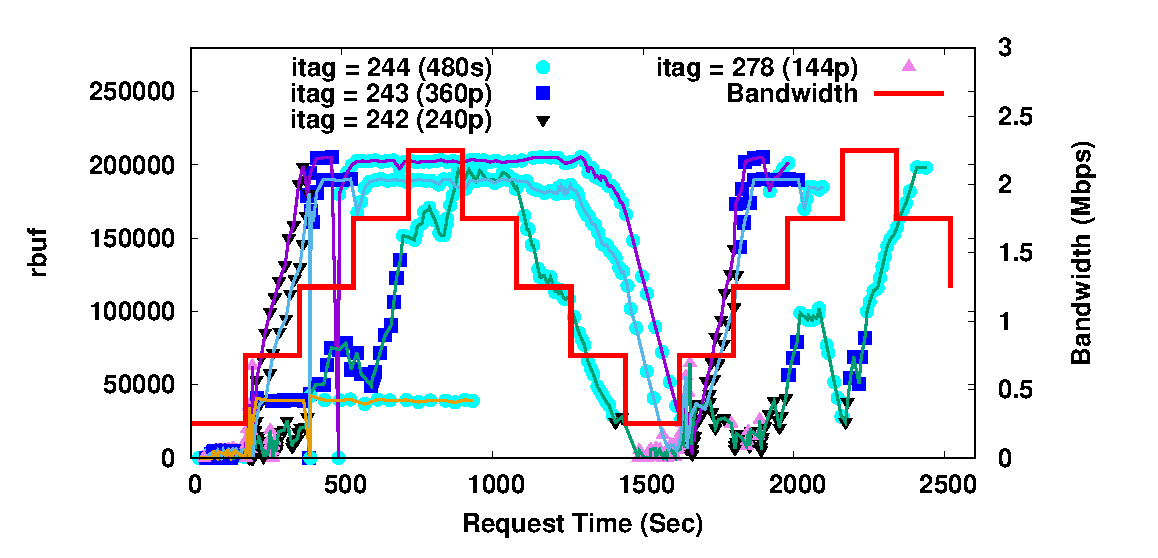
\includegraphics[width=0.7\linewidth]{img/plot_rbuf_analysis.eps}
  \caption{\small{$rbuf$ evolution}}
  \label{fig:chap03s1:rbuf_evol}
\end{figure}
\begin{figure}[!h]
 \centering
  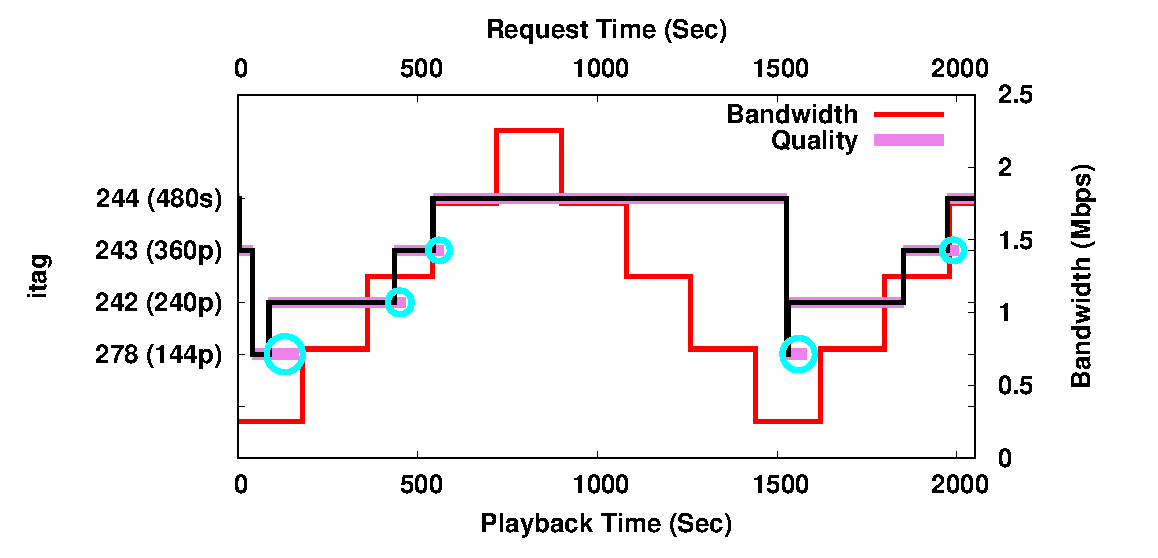
\includegraphics[width=0.7\linewidth]{img/plot_timerange}
  \caption{\small{$itag$ evolution}}
  \label{fig:chap03s1:timespent}
\end{figure}
\begin{figure}[!h]
 \centering
  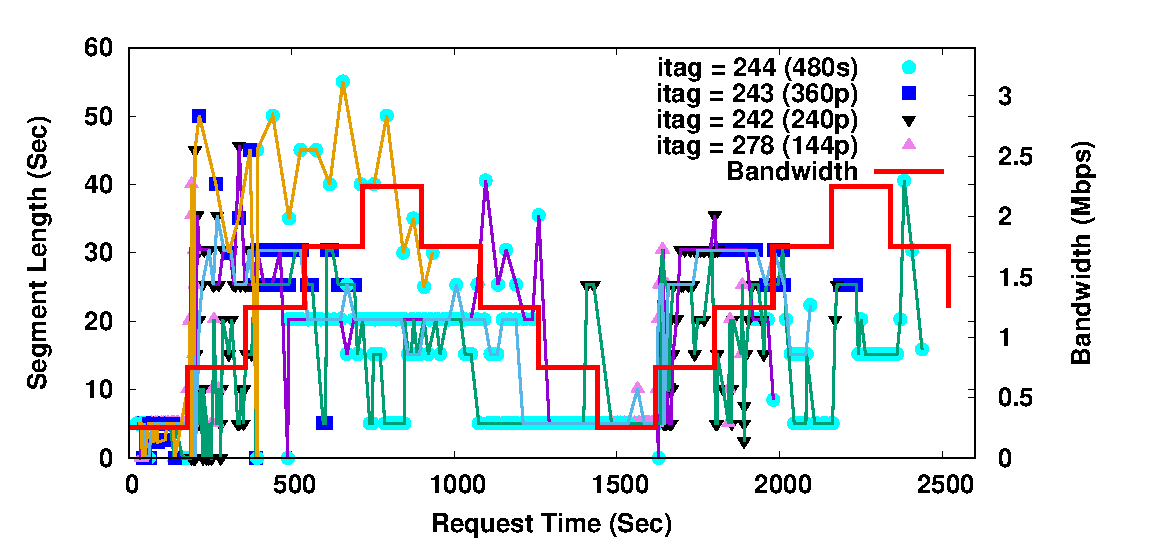
\includegraphics[width=0.7\linewidth]{img/plot_seg_comb}
  \caption{\small{Segment length adaptation}}
  \label{fig:chap03s1:segmentLength}
\end{figure}

{\bf {\em rn}:} Our experiments unveil that $rn$ is non-decreasing for a video session.
%
By observing the sequence of \ac{HTTP} requests sent by the YouTube client to YouTube server, we conclude that $rn$ is the request number to uniquely identify a \ac{DASH} video playback request.

{\bf {\em rbuf}:} We plot evolution of $rbuf$ for $4$ videos and the corresponding $itag$ values in \fig\ref{fig:chap03s1:rbuf_evol} with varying link bandwidth.
In the figure, the lines denote results for the different videos, while color codes are used to distinguish between $itag$ values.
Each point in the graph corresponds to a video playback request sent from the YouTube client.
We observe that $rbuf$ increases as the YouTube client fetches more data from the server, while it depletes if there is no request from the client to the server.
Further, whenever $rbuf$ starts decreasing, the client starts fetching data for a different $itag$ value (as we observe near $1600$ secs).
Also, as bandwidth increases, $rbuf$ keeps on increasing until it reaches a threshold, and then remains constant.
Conversely, as bandwidth drops, $rbuf$ either remains constant or diminishes.
The observations obviate that $rbuf$ denotes the {\it receive buffer} at the client.

\begin{table}[!t]
 \caption{\small{Evolution of $range$ across $rn$ and the corresponding $itag$, \textbf{payload} is in bytes}}
\label{table:chap03s1:itag-rng}
 \small
 \centering
 \csvreader[tabular=|c|c|c|c||c|c|c|c|,
    table head=\hline \bfseries rn & \bfseries itag & \bfseries range & \bfseries Payload & \bfseries rn & \bfseries itag & \bfseries range & \bfseries Payload \\\hline,
    table foot=\hline]%
{\relpath/csv/itag-rng.csv}{}%
{\csvcoli & \csvcolii & \csvcoliii & \csvcoliv & \csvcolv & \csvcolvi & \csvcolvii & \csvcolviii}%
% \csvautotabular{csv/itag-rng.csv}
\end{table}

{\bf {\em range}:} \tbl\ref{table:chap03s1:itag-rng} presents sample values of $range$ for a particular video.
The $range$ values consist of two integers separated by `-'; the first integer is always smaller than the second one -- therefore, the two integers indicate $start$ and $end$ of a $range$ value.
We also observe that the sizes of the response payloads are given by ($end - start + 1$).
We conclude that $range$ is the byte range parameter in \ac{HTTP} request header.
As a proof of concept, we also perform the following experiment:
YouTube provides an \ac{API} called \texttt{get\_video\_info} through the \ac{URL}~\url{https://www.youtube.com/get_video_info?video_id=<video_ID>} -- the \ac{API} provides information regarding $itag$ values used in a video, as well as URLs to download a complete video (with unrestricted access), or video chunks (using $range$) for a particular $itag$.
Using the \ac{API}, we download the video chunks of different videos for different available $itag$ values.
Then for these videos, we also download different video chunks using the \texttt{wget} utility, by changing the values of the $range$ parameter.
We observe that \acsu{MD5}\cite{rfc1321_md5} checksums of the downloaded video chunks for a $itag$ value are equal to the \acsu{MD5} checksum of the byte range of the original video of that particular $itag$.
This reinforces our conclusion that $range$ indicates \ac{HTTP} byte range; YouTube client adaptively changes this parameter to increase or decrease the video chunk size to be fetched, based on network conditions.

{\bf {\em clen}:} In order to interpret the significance of $clen$, we start a browser with developer mode enabled and start monitoring network activities.
We render a video in YouTube client and collect the video playback request \acp{URL}.
We then change the value of the $range$ parameter with $4$ different cases where $range$ is equal to (a) [$0$, $clen$],  (b) [$0$, $(clen-x)$] where $0<x<clen$ is some positive random number, (c) [$0$, $(clen+x)$], and (d) with the range parameter omitted.
Chunks are fetched from these \acp{URL} using \texttt{wget} command and the lengths and \acsu{MD5} checksums of the received data segments are checked.
We observe that for a particular $itag$, (i) the length and MD5 checksum of the received data are exactly same for the cases when  $range$ is omitted or $range$ is either [$0$, $clen$] or [$0$, $(clen+x)$] -- in such cases, the length of the data is $clen$.
However, the length of the data is $clen-x$ when the range value is [$0$, $(clen-x)$].
We observe similar behavior across all videos that we randomly chose.
From these observations, we conclude that $clen$ is the length of the video chunk for a particular $itag$ value.
The YouTube server stores a video chunk with $clen$ amount of data for a particular $itag$, and therefore the length of received data never shoots beyond $clen$ even if the byte range requested through $range$ is higher.

\subsubsection{Summary} $range$ and $itag$ are parameters responsible for adaptiveness in YouTube video streaming, while $rbuf$ is the client-side indicator of channel quality.
Although the maximum length of a video segment is defined by $clen$ for a particular $itag$, YouTube has the option to download lesser data per request, which is specified by the $range$ parameter.

\section{Insights into YouTube's Bitrate Adaptation Algorithm}
\label{chap03s1:subsec:seglength}
Based on the above analysis of various parameters, we figure out various important aspects of YouTube's \acr{ABR} algorithm, as follows.

\subsection{Opportunistic (Quality) Upscale vs. Conservative Downscale} We concentrate on the nature of YouTube video playback requests whenever it switches from one video quality to another.
We first convert the $range$ parameter to equivalent video segment length in terms of video playback time -- this can be done by looking into the video file header (using the Python package \texttt{python-ebml}) that provides a mapping between the byte range and playback time.
\fig\ref{fig:chap03s1:timespent} plots the video segments (in terms of video playback time, as shown in x-axis) and the corresponding $itag$ values for which the client makes a request.
We make an interesting observation -- whenever the video quality improves, there is an overlap between the segments of lower quality and higher quality (shown using circles in the figure); however, there is no such overlap when the video quality drops.
Therefore, we can conclude that the YouTube video adaptation algorithm works in a way where it takes an opportunistic approach for downloading higher quality video segments when the link quality improves, but takes a conservative approach when the link quality drops.
In the opportunistic approach, it downloads the video chunks of both the video qualities in parallel, whenever it decides to switch from the lower quality to the higher quality -- this often leads to data wastage, as mentioned earlier in \S\ref{chap03s1:sec:introduction}.
However, in the conservative approach, it directly sends the request for lower quality video when the link quality drops.

\subsection{Segment Length Adaptation}
As mentioned earlier, YouTube adapts both the video quality and the streaming data rate whenever network conditions change.
In order to explore the behavior of streaming data rate adaptation, we analyze how the requested video segment length (specified by the $range$ parameter) per video playback request, changes with change in link bandwidth.
We convert the byte range mentioned in the video playback request to the equivalent video playback time, and find out the video segment length in terms of playback time.
The sample results from $4$ videos are shown in \fig\ref{fig:chap03s1:segmentLength} where x-axis denotes the video playback request time, and y-axis denotes the segment length in seconds.
We use different color codes to indicate the $itag$ values associated with corresponding playback requests.
The figures give very interesting insights into YouTube video streaming behavior -- whenever the link bandwidth increases, YouTube first increases the segment length of lower quality video and buffers maximum amount of video data.
It then switches to the higher quality video but with smaller segment lengths.
At this point, we observe an overlap between the segments of two different video qualities, as discussed earlier with \fig\ref{fig:chap03s1:timespent}.
Then it progressively increases the segment length and repeats the procedure for the next higher quality level video if the link quality improves further (measured through the increase rate of $rbuf$).
However, when the link quality drops, in a similar way, YouTube first starts requesting for same quality video chunks of smaller segments, and drops the segment length.
If it still observes a drop in $rbuf$ after reducing the segment length in the playback requests, then it switches to request for the next lower quality level video chunks of smaller segments.
Segment length is increased only if $rbuf$ becomes stable.
In this manner, YouTube jointly adapts the video quality as well as the segment length (indirectly, the streaming data rate).
This observation has not been reported in existing literature, to the best of our knowledge.

\subsection{Implication on Data Wastage}
Segment length adaptation may have far-reaching implications in terms of advantages for YouTube streaming, one of which is minimal data wastage.
Since segment length increases gradually from a low value to higher values when bandwidth improves, overlaps between the segments of a lower quality and the next higher quality are largely diminished.
This implies that data wastage values come down drastically (as opposed to a scenario with no segment length adaptation) -- in our experiments, we compute the average wastage ratio, defined as $\frac{data\_downloaded - data\_played}{data\_played}$, to be $0.82 x 10^{-6}$.
This is in sharp contrast with previously reported values.

